%%%%%%%%%%%%%%%%%%%%%%%%%%%%%%%%%%%%%%%%%%%%%%%%%%%%%%%%%%%%%%%%%%%%%%%%%%%%%%%%
%2345678901234567890123456789012345678901234567890123456789012345678901234567890
%        1         2         3         4         5         6         7         8

% Comment this line out if you need a4paper
\documentclass[letterpaper, 10 pt, conference]{ieeeconf}  

% Use this line for a4 paper
%\documentclass[a4paper, 10pt, conference]{ieeeconf}

% This command is only needed if you want to use the \thanks command
\IEEEoverridecommandlockouts

% Needed to meet printer requirements.
\overrideIEEEmargins

%In case you encounter the following error:
%Error 1010 The PDF file may be corrupt (unable to open PDF file) OR
%Error 1000 An error occurred while parsing a contents stream. Unable to analyze the PDF file.
%This is a known problem with pdfLaTeX conversion filter. The file cannot be opened with acrobat reader
%Please use one of the alternatives below to circumvent this error by uncommenting one or the other
%\pdfobjcompresslevel=0
%\pdfminorversion=4

% See the \addtolength command later in the file to balance the column lengths
% on the last page of the document

% Imports
\usepackage{amsmath}
\usepackage{amsfonts}
%\usepackage{amsthm} % Errors from \proof when used with this ieeeconf
\usepackage{mathtools}
%\usepackage{flushend} % Sometimes breaks order of references
% Algorithms
\usepackage{algorithm}
\usepackage{algpseudocode}
\usepackage{setspace}
% Graphics
\usepackage{tikz}
% Local
\usepackage{local_macros/isasmathmacros}
% \usepackage{lmodern}

% Environments
%\theoremstyle{definition} % Doesn't exist when used with this ieeeconf
\newtheorem{definition}{Definition}[section]
\newtheorem{theorem}{Theorem}[section]

%\theoremstyle{remark} % Doesn't exist when used with this ieeeconf
%\newtheorem*{remark}{Remark} % Doesn't exist when used with this ieeeconf
\newtheorem{remark}{Remark}

% Tiks colours
\definecolor{pyplotblue}{RGB}{31,119,180}
\definecolor{pyplotorange}{RGB}{255,127,14}
\definecolor{pyplotgreen}{RGB}{44,160,44}

% Algorithm settings
\algnewcommand{\LineComment}[1]{\Statex \(\triangleright\) #1}

\title{\LARGE \bf
Encrypted Fast Covariance Intersection\\Without Leaking Fusion Weights
}

\author{Marko Ristic$^{1}$ and Benjamin Noack$^{1}$% <-this % stops a space
\thanks{$^{1}$Marko Ristic and Benjamin Noack are with the Autonomous Multisensor Systems Group (AMS), Institute for Intelligent Cooperating Systems (ICS), Otto von Guericke University (OVGU), Magdeburg, Germany {\tt\small \{marko.ristic, benjamin.noack\}@ovgu.de}}%
}

\begin{document}

\maketitle
\thispagestyle{empty}
\pagestyle{empty}

%%%%%%%%%%%%%%%%%%%%%%%%%%%%%%%%%%%%%%%%%%%%%%%%%%%%%%%%%%%%%%%%%%%%%%%%%%%%%%%%
% 
%        d8888 888888b.    .d8888b.  
%       d88888 888  "88b  d88P  Y88b 
%      d88P888 888  .88P  Y88b.      
%     d88P 888 8888888K.   "Y888b.   
%    d88P  888 888  "Y88b     "Y88b. 
%   d88P   888 888    888       "888 
%  d8888888888 888   d88P Y88b  d88P 
% d88P     888 8888888P"   "Y8888P"  
%                                    
%                                    
%                                    
% 
\begin{abstract}
    State estimate fusion is a common requirement in distributed sensor networks and can be complicated by untrusted participants or network eavesdroppers. We present a method for computing the common Fast Covariance Intersection fusion algorithm on an untrusted cloud without disclosing individual estimates or the fused result. In an existing solution to this problem, fusion weights corresponding to the sensor estimate errors are leaked to the cloud to perform the fusion. In this work, we present a method that guarantees no data identifying sensors or their estimated values is leaked to the cloud by requiring an additional computation step by the party querying the cloud for the fused result. The Paillier encryption scheme is used to homomorphically compute separate parts of the computation that can be combined after decryption. This encrypted Fast Covariance Intersection algorithm can be used in scenarios where the fusing cloud is not trusted and any information on sensor performances must remain confidential.
\end{abstract}

%%%%%%%%%%%%%%%%%%%%%%%%%%%%%%%%%%%%%%%%%%%%%%%%%%%%%%%%%%%%%%%%%%%%%%%%%%%%%%%%

% 
% 8888888 888b    888 88888888888 8888888b.   .d88888b.  
%   888   8888b   888     888     888   Y88b d88P" "Y88b 
%   888   88888b  888     888     888    888 888     888 
%   888   888Y88b 888     888     888   d88P 888     888 
%   888   888 Y88b888     888     8888888P"  888     888 
%   888   888  Y88888     888     888 T88b   888     888 
%   888   888   Y8888     888     888  T88b  Y88b. .d88P 
% 8888888 888    Y888     888     888   T88b  "Y88888P"  
%                                                        
%                                                        
%                                                        
% 
\section{Introduction}\label{sec:introduction}
Data fusion and distributed state estimation have long been active fields of research and continue to find many applications in modern systems today \cite{andersonOptimalFiltering1979,simonOptimalStateEstimation2006}. Methods relying on the Kalman filter and derivatives \cite{haugBayesianEstimationTracking2012} have become particularly prevalent in this area due to their recursive structure and suitability to modelling estimate cross-correlations typically required for data fusion \cite{mutambaraDecentralizedEstimationControl1998,ligginsDistributedDataFusion2012}. The handling of these cross-correlations is especially important when consistent or optimal fusion is desired \cite{bar-shalomTracktotrackCorrelationProblem1981,sunMultisensorOptimalInformation2004} and presents a key challenge in data fusion when they are not known in advance. To overcome this, some methods propagate cross-correlations through time at the cost of repeated reconstruction \cite{steinbringOptimalSamplebasedFusion2016,radtkeReconstructionCrossCorrelationsConstant2018,radtkeFullyDecentralizedEstimationUsing2021} and typically add local computational complexity. Alternative methods approximate error cross-correlations with conservative suboptimal estimates to provide consistent fusion instead \cite{julierNondivergentEstimationAlgorithm1997,noackDecentralizedDataFusion2017,niehsenInformationFusionBased2002}. One such popular method is Covariance Intersection \cite{julierNondivergentEstimationAlgorithm1997} and its computationally inexpensive approximation, Fast Covariance Intersection \cite{niehsenInformationFusionBased2002}. These methods minimise fusion estimate error given possible conservative estimates and are popular due to their compatibility with the information form of the Kalman filter \cite{mutambaraDecentralizedEstimationControl1998,pfaffInformationFormDistributed2017}.
% Figure moved here arbitrarily to be on the top right corner of the first page.
\begin{figure}[t]
    \centering
    % \begin{tikzpicture}
    %     % Bounding box
    %     %\draw [gray] (1,-1.5) rectangle (8.5,7);
    %     % Estimators
    %     \node at (2.5,6.25) {Estimator $1$};
    %     \node at (7,6.25) {Estimator $m$};
    %     \fill [pyplotorange!70] (7,5.5) ellipse (0.5 and 0.5);
    %     \fill [pyplotorange!70] (2.5,5.5) ellipse (0.5 and 0.5);
    %     \fill [black] (5,5.5) circle (0.05);
    %     \fill [black] (4.5,5.5) circle (0.05);
    %     \fill [black] (4.75,5.5) circle (0.05);
    %     % Estimates
    %     \node [right] at (6.25,4.5) {$\hat{\vec{x}}_{k,m},\mat{P}_{k,m}$};
    %     \node [left] at (3.25,4.5) {$\hat{\vec{x}}_{k,1},\mat{P}_{k,1}$};
    %     % Fusion
    %     \node [right] at (5.25,0.5) {$\hat{\vec{x}}_{k,\mathsf{fus}},\mat{P}_{k,\mathsf{fus}}$};
    %     % Cloud
    %     \node at (4.75,3.65) {Cloud};
    %     \fill [pyplotorange!70] (4.75,3) ellipse (0.4 and 0.4);
    %     \fill [pyplotorange!70] (5.25,2.75) ellipse (0.4 and 0.25);
    %     \fill [pyplotorange!70] (4.25,2.75) ellipse (0.25 and 0.25);
    %     \fill [pyplotorange!70] (5.25,3) ellipse (0.25 and 0.25);
    %     \fill [pyplotorange!70] (4.25,2.5) rectangle (5.25,2.75);
    %     % Third-party
    %     \node at (4.75,1.25) {Trusted Third-party};
    %     \fill [pyplotblue!70] (5.5,-0.25) -- (4,-0.25) -- (4.75,1);
    %     % Estimator arrows
    %     \draw [-latex]  plot coordinates {(3,5)  (4.25,4)};
    %     \draw [-latex]  plot coordinates {(6.5,5)  (5.25,4)};
    %     % Third-party arrows
    %     \draw [latex-latex]  plot coordinates {(4.75,2.3)  (4.75,1.65)};
    % \end{tikzpicture}
    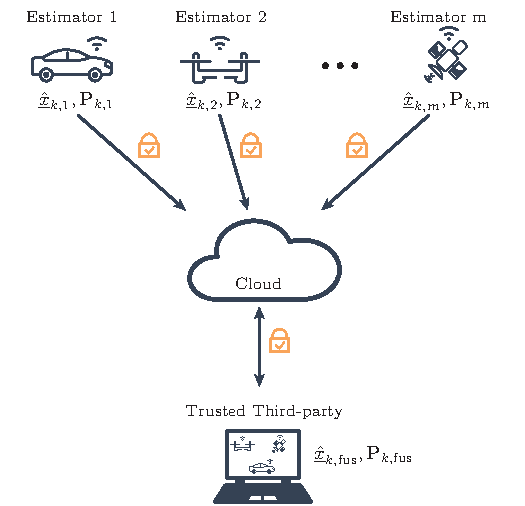
\includegraphics[width=\columnwidth]{figures/illustration.pdf}%
    \caption{The participants, inputs and output of the considered fusion scenario.}\vspace{-\baselineskip}%
    \label{fig:layout}%
\end{figure}%

While effective and often efficient, these data fusion solutions have traditionally been performed on closed networks with trusted participants and inherently imply trust between sensors and estimators. In recent years, the ubiquity of distributed public networks has seen the additional challenges of security and privacy become increasingly relevant in distributed sensing environments and has led to an active field of research in providing security during data processing and fusion tasks \cite{renSecurityChallengesPublic2012,brennerSecretProgramExecution2011}. While one can ensure transmitted information is kept secret from eavesdroppers on untrusted networks by using common private and public key encryption schemes \cite{katzIntroductionModernCryptography2008}, tasks involving untrusted participants during computations present a greater challenge. Here, partial computations on encrypted data or the intended leakage of some results are often required or desired to arrive at the final result \cite{risticSecureFastCovariance2021,shiPrivacyPreservingAggregationTimeSeries2011,risticCryptographicallyPrivilegedState2022}. One common tool for achieving these requirements is homomorphic encryption \cite{gentryFullyHomomorphicEncryption2009,paillierPublicKeyCryptosystemsBased1999} which allows operations to be computed on encrypted numbers without decryption. The Pailler encryption scheme \cite{paillierPublicKeyCryptosystemsBased1999} allows homomorphic addition and is a frequent choice in fusion applications due to its applicability, simplicity and provable security. In \cite{alanwarPrOLocResilientLocalization2017}, the Paillier scheme is used to perform non-Bayesian measurement fusion with range-sensors without disclosing individual sensor locations or measurements, while in \cite{aristovEncryptedMultisensorInformation2018}, it is used to achieve similar security with a Kalman filter when measurements are linear and sensors form a hierarchical network. When paired with additional schemes that introduce some leakage, a wider variety of tasks can often be solved as well. The work in \cite{alexandruEncryptedCooperativeControl2019} uses private weighted sum aggregation together with the Paillier scheme to compute decentralised local control inputs while leaking only the sum of weighted neighbouring states, and in \cite{risticSecureFastCovariance2021}, an untrusted cloud can use order-revealing encryptions to compute and leak relative sensor accuracies allowing the homomorphic computation of the Fast Covariance Intersection algorithm.

In this work, we consider stochastic state estimate fusion on an untrusted cloud similar to \cite{risticSecureFastCovariance2021} but aim to fuse estimates without leaking sensor information at the cloud. Our contribution is a novel method for computing the Fast Covariance Intersection algorithm using only the Paillier encryption scheme and leaking no intermediate information to the untrusted cloud. While in some use cases, leaked relative sensor accuracies can be useful for prioritising sensor communications, this leakage inherently informs the cloud about sensor performances over time, disclosing the times when sensors are out of range or non-functioning and implicitly leaking information about the fused estimate. Therefore, the presented method finds application when all sensor information is considered sensitive and when the fusing cloud is not trusted.

Section~\ref{sec:problem} introduces the formal data fusion and security goals and section~\ref{sec:prelims} gives relevant preliminaries. Section~\ref{sec:encrypted_fci} introduces our method, before sections~\ref{sec:security} and \ref{sec:simulation} analyse its security and simulation results, respectively. Concluding remarks and future work are discussed in section~\ref{sec:conclusion}.

\subsection{Notation}
Throughout this work, the following notation is used. Plain characters, $a$, denote scalars, underlined lowercase characters, $\vec{b}$, denote vectors and uppercase bold characters, $\mat{C}$, denote matrices. $\vec{0}$ denotes the zero vector, $\mat{C}^{-1}$ the matrix inverse and $\tr(\mat{C})$ the matrix trace. Encryption with a public key $\mathsf{pk}$ is denoted $\mathcal{E}_{\mathsf{pk}}(\cdot)$ and decryption with a private key $\mathsf{sk}$ is denoted $\mathcal{D}_{\mathsf{sk}}(\cdot)$, while integer encoding and decoding with parameters $M$ and $\phi$ are denoted $\mathsf{E}_{M,\phi}(\cdot)$ and $\mathsf{E}^{-1}_{M,\phi}(\cdot)$, respectively. All encryption and encoding operations on vectors or matrices are performed element-wise and the expression $\otimes_{i=1}^{m}\mat{C}_i$ is used to denote element-wise multiplication for multidimensional data. The function $\mathsf{lcm}(a_1,a_2)$ gives the lowest common denominator of integers $a_1$ and $a_2$, $\lfloor\cdot\rfloor$ denotes rounding towards zero and $\lfloor\cdot\rceil$ denotes rounding to the nearest integer. The set $\mathbb{Z}_N$ is the set of integers modulo $N$ and $\pmod{N}$ the associated modulo-$N$ operation.

% 
% 8888888b.  8888888b.   .d88888b.  888888b.   
% 888   Y88b 888   Y88b d88P" "Y88b 888  "88b  
% 888    888 888    888 888     888 888  .88P  
% 888   d88P 888   d88P 888     888 8888888K.  
% 8888888P"  8888888P"  888     888 888  "Y88b 
% 888        888 T88b   888     888 888    888 
% 888        888  T88b  Y88b. .d88P 888   d88P 
% 888        888   T88b  "Y88888P"  8888888P"  
%                                              
%                                              
%                                              
% 
\section{Problem Statement}\label{sec:problem}
In this work, we consider an arbitrary time-varying process defined by its state $\vec{x}_k \in \mathbb{R}^n$ for all timesteps $k \in \mathbb{N}$. This process is estimated by $m$ individual estimators $i$, $1\leq i\leq m$, each producing a state estimate and an estimate error covariance,
\begin{equation}\label{eqn:ests_and_covs}
    \hat{\vec{x}}_{k,i} \in \mathbb{R}^n \text{ and } \mat{P}_{k,i} \in \mathbb{R}^{n\times n}\,,
\end{equation}
respectively, at every timestep $k$. Our aim at every timestep is for all estimates $\hat{\vec{x}}_{k,i}$ and errors $\mat{P}_{k,i}$, $1\leq i\leq m$, to be sent to a cloud server where a fused estimate and error covariance,
\begin{equation}\label{eqn:fus_ests_and_covs}
    \hat{\vec{x}}_{k,\mathsf{fus}} \in \mathbb{R}^n \text{ and } \mat{P}_{k,\mathsf{fus}} \in \mathbb{R}^{n\times n}\,,
\end{equation}
respectively, are computed and are consistent with the estimates in \eqref{eqn:ests_and_covs}.

Simultaneously, we consider the desired security of the fusion process. The fusing cloud and estimators are treated as \textit{honest-but-curious}, that is, they follow protocols correctly but may use learned information for malicious gain, and a trusted third-party exists that can query the cloud at any timestep $k$ to obtain the fusion results in \eqref{eqn:fus_ests_and_covs}. We aim for the cloud, estimators and eavesdroppers to learn no additional information from observed estimates and fusions, \eqref{eqn:ests_and_covs} and \eqref{eqn:fus_ests_and_covs}, respectively, beyond their local estimates. To guarantee this, cryptographic \textit{Indistinguishability under the Chosen Plaintext Attack} (IND-CPA) \cite{katzIntroductionModernCryptography2008} is desired for all transmitted and processed information. This is in line with common security goals in the field and is suitable for homomorphic encryption. The communications of this scenario are summarised graphically in figure \ref{fig:layout}.

% 
% 8888888b.  8888888b.  8888888888 888      8888888 888b     d888 
% 888   Y88b 888   Y88b 888        888        888   8888b   d8888 
% 888    888 888    888 888        888        888   88888b.d88888 
% 888   d88P 888   d88P 8888888    888        888   888Y88888P888 
% 8888888P"  8888888P"  888        888        888   888 Y888P 888 
% 888        888 T88b   888        888        888   888  Y8P  888 
% 888        888  T88b  888        888        888   888   "   888 
% 888        888   T88b 8888888888 88888888 8888888 888       888 
%                                                                 
%                                                                 
%                                                                 
% 
\section{Preliminaries}\label{sec:prelims}
When proposing our solution in section~\ref{sec:encrypted_fci}, we make use of the Fast Covariance Intersection algorithm, the Paillier homomorphic encryption scheme and a common integer encoding for floating-point numbers. These preliminaries are summarised below.

\subsection{Fast Covariance Intersection}\label{subsec:fci}
The Fast Covariance Intersection (FCI) algorithm \cite{niehsenInformationFusionBased2002} provides a consistent suboptimal fusion of estimates in the form \eqref{eqn:ests_and_covs} when cross-correlations between the measurements are not known, providing a fast, non-iterative and general solution. Fusion is given by
\begin{equation}\label{eqn:ci_cov_fusion}
    \mat{P}_{k,\mathsf{fus}} = \left(\sum_{i=1}^m\omega_{k,i}\mat{P}_{k,i}^{-1}\right)^{-1}
\end{equation}
and
\begin{equation}\label{eqn:ci_est_fusion}
    \hat{\vec{x}}_{k,\mathsf{fus}} = \mat{P}_{k,\mathsf{fus}}\sum_{i=1}^m\omega_{k,i}\mat{P}_{k,i}^{-1}\hat{\vec{x}}_{k,i}\,,
\end{equation}
with positive fusion weights $\omega_{k,i} \in \mathbb{R}^{+}$, $1\leq i \leq m$, such that 
\begin{equation}
    \sum_{i=1}^m\omega_{k,i}=1
\end{equation}
at each timestep $k$. In FCI, these weights are computed non-iteratively, as
\begin{equation}\label{eqn:fci_weights}
    \omega_{k,i} = \frac{1/\tr(\mat{P}_{k,i})}{\sum_{i=1}^m 1/\tr(\mat{P}_{k,i})}\,.
\end{equation}

\subsection{Paillier Encryption Scheme}\label{subsec:paillier}
The Paillier encryption scheme \cite{paillierPublicKeyCryptosystemsBased1999,katzIntroductionModernCryptography2008} is an additively homomorphic encryption scheme meeting the IND-CPA security notion. Key generation of the scheme is performed by choosing two sufficiently large primes of an equal bit length, $p$ and $q$, and computing $N=pq$. The public key is defined by $\mathsf{pk} \coloneqq N$ and the private key by $\mathsf{sk} \coloneqq (p,q)$.

Encryption of a plaintext message $a \in \mathbb{Z}_N$, resulting in a ciphertext $\mathcal{E}_\mathsf{pk}(a) \in \mathbb{Z}^*_{N^2}$, is computed by
\begin{equation}
    \mathcal{E}_\mathsf{pk}(a) = (N+1)^a r^N \pmod{N^2}
\end{equation}
with a randomly chosen $r \in \mathbb{Z}_N$. The decryption of the ciphertext is computed by
\begin{equation}
    \mathcal{D}_\mathsf{sk}(\mathcal{E}_\mathsf{pk}(a)) = \frac{L\left(\mathcal{E}_\mathsf{pk}(a)^\lambda \pmod{N^2}\right)}{L\left((N+1)^\lambda \pmod{N^2}\right)}\pmod{N}
\end{equation}
where $\lambda = \mathsf{lcm}(p-1,q-1)$ and $L(u)=\frac{u-1}{N}$. In addition to encryption and decryption, the following homomorphic properties are provided by the Paillier encryption scheme. $\forall a_1,a_2 \in \mathbb{Z}_N$,
\begin{align}
    \begin{split}\label{eqn:paillier_add}
        \mathcal{D}_\mathsf{sk}(\mathcal{E}_\mathsf{pk}(a_1)\mathcal{E}_\mathsf{pk}(a_2) & \pmod{N^2})\\
        &= a_1+a_2 \pmod{N}\,,
    \end{split}\\
    \begin{split}\label{eqn:paillier_add_known}
        \mathcal{D}_\mathsf{sk}(\mathcal{E}_\mathsf{pk}(a_1)(N+1)^{a_2} & \pmod{N^2})\\
        &= a_1+a_2\pmod{N}\,,
    \end{split}\\
    \begin{split}
        \mathcal{D}_\mathsf{sk}(\mathcal{E}_\mathsf{pk}(a_1)^{a_2} & \pmod{N^2})\\
        &= a_1a_2 \pmod{N}\,.
    \end{split}
\end{align}

\subsection{Integer Encoding for Homomorphic Encryption}\label{subsec:encoding}
As the Paillier scheme bounds inputs to $a\in \mathbb{Z}_N$, multidimensional real-valued state estimates and error covariances require a suitable integer mapping to allow for their encryption and to preserve homomorphic operations. We achieve this with element-wise encoding and encryption, and rely on a generalised Q number encoding \cite{oberstarFixedPointRepresentationFractional2007}. Parametrised by a range $M\in \mathbb{N}$ and a fractional precision $\phi \in \mathbb{N}$, the encoding of a number $x\in\mathbb{R}$ is given by
\begin{equation}
    \mathsf{E}_{M,\phi}(x) = \left\lfloor \phi x \right\rceil \pmod{M}\,,
\end{equation}
while decoding of an encoded number $u\in\mathbb{Z}_M$ is given by
\begin{equation}
    \mathsf{E}^{-1}_{M,\phi}(u) =
    \begin{dcases}
        \frac{u \hspace{-8pt}\pmod{M}}{\phi}, &u \hspace{-8pt}\pmod{M} \leq \left\lfloor\frac{M}{2}\right\rfloor \\
        -\frac{M - u \hspace{-8pt}\pmod{M}}{\phi}, & \text{otherwise} \\
    \end{dcases}.
\end{equation}
This encoding provides the homomorphic property
\begin{equation}\label{eqn:encoding_add}
    \begin{split}
        \mathsf{E}_{M,\phi}(a_1) + \mathsf{E}_{M,\phi}(a_2)& \pmod{M}\\
        &= \mathsf{E}_{M,\phi}(a_1+a_2)
    \end{split}
\end{equation}
for $a_1,a_2\in\mathbb{R}$ when
\begin{equation}\label{eqn:encoding_overflow_req}
    \left|\phi(a_1+a_2)\right| < \left\lfloor \frac{M}{2} \right\rfloor\,.
\end{equation}
Here, we note that when $M=N$, \eqref{eqn:encoding_add} coincides with the Paillier homomorphic operations \eqref{eqn:paillier_add} and \eqref{eqn:paillier_add_known}, while when $N$ is very large ($N>2^{1024})$, \eqref{eqn:encoding_overflow_req} can generally be ignored.

% 
% 888b     d888 8888888888 88888888888 888    888  .d88888b.  8888888b.  
% 8888b   d8888 888            888     888    888 d88P" "Y88b 888  "Y88b 
% 88888b.d88888 888            888     888    888 888     888 888    888 
% 888Y88888P888 8888888        888     8888888888 888     888 888    888 
% 888 Y888P 888 888            888     888    888 888     888 888    888 
% 888  Y8P  888 888            888     888    888 888     888 888    888 
% 888   "   888 888            888     888    888 Y88b. .d88P 888  .d88P 
% 888       888 8888888888     888     888    888  "Y88888P"  8888888P"  
%                                                                        
%                                                                        
%                                                                        
% 
\section{Encrypted Fast Covariance Intersection}\label{sec:encrypted_fci}
With the problem and preliminaries introduced, we can now present our encrypted FCI method that leaks no information to the fusing cloud. The core idea behind the method is to postpone the evaluation of operations that cannot be performed homomorphically until partial results are queried and decrypted by the key-holding third-party. The remaining operations can then be evaluated on unencrypted inputs to produce the correct results.

First, we note that the FCI fusion equations \eqref{eqn:ci_cov_fusion} and \eqref{eqn:ci_est_fusion} can be rearranged and substituted with weights \eqref{eqn:fci_weights} to obtain the equations
\begin{equation}\label{eqn:fci_cov_rearrange}
    \mat{P}_{k,\mathsf{fus}} = \left(\left(\sum_{i=1}^m \frac{1}{\tr(\mat{P}_{k,i})}\right)^{-1}\sum_{i=1}^m \frac{1}{\tr(\mat{P}_{k,i})}\mat{P}_{k,i}^{-1}\right)^{-1}
\end{equation}
and
\begin{equation}\label{eqn:fci_est_rearrange}
    \hat{\vec{x}}_{k,\mathsf{fus}} = \mat{P}_{k,\mathsf{fus}}\left(\sum_{i=1}^m \frac{1}{\tr(\mat{P}_{k,i})}\right)^{-1}\sum_{i=1}^m\frac{1}{\tr(\mat{P}_{k,i})}\mat{P}_{k,i}^{-1}\hat{\vec{x}}_{k,i}\,.
\end{equation}
In this form, innermost summations  
\begin{equation}
    \begin{split}
        \sum_{i=1}^m \frac{1}{\tr(\mat{P}_{k,i})}\,,\ \sum_{i=1}^m &\frac{1}{\tr(\mat{P}_{k,i})}\mat{P}_{k,i}^{-1}\text{ and }\\ 
        &\qquad\sum_{i=1}^m\frac{1}{\tr(\mat{P}_{k,i})}\mat{P}_{k,i}^{-1}\hat{\vec{x}}_{k,i}
    \end{split}
\end{equation}
combine information from individual estimators $i$ and are computable homomorphically given suitable encryptions. Encryptions of these sums can then be decrypted by the key-holding third-party, before remaining inversions and multiplications in \eqref{eqn:fci_cov_rearrange} and \eqref{eqn:fci_est_rearrange} can be computed to obtain the final results. To depict this process, pseudocode for the encryption at estimators, fusion at the cloud and decryption by the third-party are provided in algorithms~\ref{alg:est_enc}, \ref{alg:cloud_fus} and \ref{alg:fus_query}, respectively.
\begin{algorithm}[htbp]
\caption{Estimator Encryption}\label{alg:est_enc}
\begin{algorithmic}[1]
    \setstretch{1.35}
    \Procedure{Estimate}{$i$, $k$, $\mathsf{pk}$, $\phi$}
    \State Estimate $\hat{\vec{x}}_{k,i}$ locally
    \State Estimate $\mat{P}_{k,i}$ locally
    \LineComment{Public key is encoding and encryption modulus}
    \State $N \gets \mathsf{pk}$
    \LineComment{Encode scaling, covariance and estimate components}
    \State $\tilde{s}_{k,i} \gets \mathsf{E}_{N,\phi}\left(\frac{1}{\tr(\mat{P}_{k,i})}\right)$
    \State $\tilde{\mat{C}}_{k,i} \gets \mathsf{E}_{N,\phi}\left(\frac{1}{\tr(\mat{P}_{k,i})}\mat{P}_{k,i}^{-1}\right)$
    \State $\tilde{\vec{e}}_{k,i} \gets \mathsf{E}_{N,\phi}\left(\frac{1}{\tr(\mat{P}_{k,i})}\mat{P}_{k,i}^{-1}\hat{\vec{x}}_{k,i}\right)$
    \LineComment{Encrypt scaling, covariance and estimate components}
    \State $s_{k,i} \gets \mathcal{E}_{\mathsf{pk}}\left(\tilde{s}_{k,i}\right)$
    \State $\mat{C}_{k,i} \gets \mathcal{E}_{\mathsf{pk}}\left(\tilde{\mat{C}}_{k,i}\right)$
    \State $\vec{e}_{k,i} \gets \mathcal{E}_{\mathsf{pk}}\left(\tilde{\vec{e}}_{k,i}\right)$
    \State Send $s_{k,i}$, $\mat{C}_{k,i}$ and $\vec{e}_{k,i}$ to fusing cloud
    \EndProcedure
\end{algorithmic}
\end{algorithm}
\begin{algorithm}[htbp]
\caption{Cloud Fusion}\label{alg:cloud_fus}
\begin{algorithmic}[1]
    \setstretch{1.35}
    \Procedure{Fuse}{$k$, $\mathsf{pk}$}
    \State Receive $s_{k,i}$, $\mat{C}_{k,i}$ and $\vec{e}_{k,i}$ for all $1\leq i \leq m$
    \State $N \gets \mathsf{pk}$
    \State $s_k \gets \prod_{i=1}^{m} s_{k,i} \pmod{N^2}$
    \State $\mat{C}_k \gets \otimes_{i=1}^{m} \mat{C}_{k,i} \pmod{N^2}$
    \State $\vec{e}_k \gets \otimes_{i=1}^{m} \vec{e}_{k,i} \pmod{N^2}$
    \State Store $s_k$, $\mat{C}_k$ and $\vec{e}_k$ in case of query
    \EndProcedure
\end{algorithmic}
\end{algorithm}
\begin{algorithm}[htbp]
\caption{Fusion Query}\label{alg:fus_query}
\begin{algorithmic}[1]
    \setstretch{1.35}
    \Procedure{GetResult}{$k$, $\mathsf{pk}$, $\mathsf{sk}$, $\phi$}
    \State Query and receive $s_k$, $\mat{C}_k$ and $\vec{e}_k$ from fusing cloud
    \State $N \gets \mathsf{pk}$
    \LineComment Decrypt
    \State $\tilde{s}_k \gets \mathcal{D}_{\mathsf{sk}}\left(s_k\right)$
    \State $\tilde{\mat{C}}_k \gets \mathcal{D}_{\mathsf{sk}}\left(\mat{C}_k\right)$
    \State $\tilde{\vec{e}}_k \gets \mathcal{D}_{\mathsf{sk}}\left(\vec{e}_k\right)$
    \LineComment Decode
    \State $\bar{s}_k \gets \mathsf{E}^{-1}_{N,\phi}\left(\tilde{s}_k\right)$
    \State $\bar{\mat{C}}_k \gets \mathsf{E}^{-1}_{N,\phi}\left(\tilde{\mat{C}}_k\right)$
    \State $\bar{\vec{e}}_k \gets \mathsf{E}^{-1}_{N,\phi}\left(\tilde{\vec{e}}_k\right)$
    \LineComment Compute Fusion
    \State $\mat{P}_{k,\mathsf{fus}} \gets \left(\bar{s}_k^{-1} \cdot \bar{\mat{C}}_k\right)^{-1}$
    \State $\hat{\vec{x}}_{k,\mathsf{fus}} \gets \mat{P}_{k,\mathsf{fus}} \cdot \bar{s}_k^{-1} \cdot \bar{\vec{e}}_k$
    \State \Return $\hat{\vec{x}}_{k,\mathsf{fus}}$, $\mat{P}_{k,\mathsf{fus}}$
    \EndProcedure
\end{algorithmic}
\end{algorithm}

\begin{remark}\label{rem:seq_extension}
    Along with allowing the summations to be performed homomorphically on the cloud, we note that this form of the FCI also allows the cloud's partial fusion operations to be evaluated sequentially. This can be seen in algorithm~\ref{alg:cloud_fus}, where individual components $s_{k,i}$, $\mat{C}_{k,i}$ and $\vec{e}_{k,i}$ from each estimator can continue to be aggregated as additional estimators send their estimate information. This, in turn, supports the dynamic joining and leaving of estimators in the network without affecting the cloud or the trusted third-party operations. The security implications of such an extension are discussed further in section~\ref{sec:security}.
\end{remark}

% 
%  .d8888b.  8888888888 .d8888b.  
% d88P  Y88b 888       d88P  Y88b 
% Y88b.      888       888    888 
%  "Y888b.   8888888   888        
%     "Y88b. 888       888        
%       "888 888       888    888 
% Y88b  d88P 888       Y88b  d88P 
%  "Y8888P"  8888888888 "Y8888P"  
%                                 
%                                 
%                                 
% 
\section{Security Analysis}\label{sec:security}
The provable security of the method in section~\ref{sec:encrypted_fci} is relatively straightforward. Our aim for IND-CPA security of all information received by the cloud, sent by the estimators or observable by eavesdroppers is achieved by the homomorphic Paillier encryption scheme. Since all transmitted information is encrypted and the cloud, estimators and eavesdroppers do not hold the secret key $\mathsf{sk}$, IND-CPA is met at all parties.

We note, however, an implicit assumption made when encrypting multidimensional data element-wise. While individual elements are indistinguishable, element-wise encryption does not encrypt the estimate's dimension $n$, which remains implicitly public. While existing methods allow the complete homomorphic encryption of vectors \cite{alexandruPrivateWeightedSum2020}, they are left for future work and considered beyond the scope of this work. Instead, we acknowledge the implicit leakage of $n$ and note that, while this may leak information about the fusion's use case, state estimates remain hidden. Additionally, intuitive extensions to the scheme, such as the dynamic joining and leaving of estimators in remark~\ref{rem:seq_extension}, may introduce further implicit leakages that must be considered if security is analysed. In this example, the periodic estimation may leak to the cloud when estimators are within an estimation range or context, and a solution may be sending dummy measurements with $s_{k,i}=\mathcal{E}_{\mathsf{pk}}(\mathsf{E}_{N,\phi}(0))$ when estimator $i$ is out of range. This extension is presented only as an example of when care needs to be taken to maintain desired security goals, but in general, extensions and solutions are task-dependent and not a focus of this work.


% 
%  .d8888b. 8888888 888b     d888 
% d88P  Y88b  888   8888b   d8888 
% Y88b.       888   88888b.d88888 
%  "Y888b.    888   888Y88888P888 
%     "Y88b.  888   888 Y888P 888 
%       "888  888   888  Y8P  888 
% Y88b  d88P  888   888   "   888 
%  "Y8888P" 8888888 888       888 
%                                 
%                                 
%                                 
% 
\section{Simulation}\label{sec:simulation}
Fusion estimates and error covariances from the encrypted FCI method in section~\ref{sec:encrypted_fci} differ from unencrypted FCI only when quantisation errors are large or summation overflow occurs. As stated in section~\ref{subsec:encoding}, when the Paillier modulus $N$ is large, these errors can often be considered negligible. In this section, we demonstrate this similarity in performance between the encrypted and unencrypted FCI fusion algorithms with a simulation. Code was written in the Python programming language, using the $\mathsf{phe}$ Paillier encryption scheme library \cite{PythonPaillier2013} and a $512$ bit length key (bit length of $N$). The simulation implements a linear constant velocity model,
\begin{equation}\label{eqn:sim_sys_model}
    \vec{x}_k =
    \begin{bmatrix}
        1 & 0.5 & 0 & 0\\
        0 & 1 & 0 & 0\\
        0 & 0 & 1 & 0.5\\
        0 & 0 & 0 & 0
    \end{bmatrix}
    \cdot \vec{x}_{k-1} + \vec{w}_k\,,
\end{equation}
with noise term $\vec{w}_k \sim \mathcal{N}(\vec{0}, \mat{Q})$ and
\begin{equation}
    \mat{Q} = 10^{-3} \cdot
    \begin{bmatrix}
        0.42 & 1.25 & 0 & 0\\
        1.25 & 5 & 0 & 0\\
        0 & 0 & 0.42 & 1.25\\
        0 & 0 & 1.25 & 5
    \end{bmatrix}\,.
\end{equation}
At each timestep $k$, the system state $\vec{x}_k$ is estimated by $m=4$ estimators, $1\leq i \leq 4$, using a standard linear Kalman filter (KF) \cite{haugBayesianEstimationTracking2012} and producing estimates and error covariances $\hat{\vec{x}}_{k,i}$ and $\mat{P}_{k,i}$, respectively. The measurements used by the KF, $\vec{z}_{k,i}$, follow the measurement models
\begin{equation}
    \vec{z}_{k,i} = 
    \begin{bmatrix}
        1 & 0 & 0 & 0\\
        0 & 0 & 1 & 0
    \end{bmatrix}
    \cdot \vec{x}_k + \vec{v}_{k,i}\,,
\end{equation}
with noise terms $\vec{v}_{k,i} \sim \mathcal{N}(\vec{0}, \mat{R}_i)$ and covariances sampled indepedently, resulting in
\begin{equation}
    \begin{split}
        &\mat{R}_1 = 
        \begin{bmatrix}
            4.77 & -0.15\\
            -0.15 & 4.94
        \end{bmatrix}\,,\ 
        \mat{R}_2 = 
        \begin{bmatrix}
            2.99 & -0.55\\
            -0.55 & 4.44
        \end{bmatrix}\,,\\
        &\mat{R}_3 = 
        \begin{bmatrix}
            2.06 & 0.68\\
            0.68 & 1.96
        \end{bmatrix}\text{ and }
        \mat{R}_4 = 
        \begin{bmatrix}
            1.17 & 0.80\\
            0.80 & 0.64
        \end{bmatrix}\,.
    \end{split}
\end{equation}
The fusion results of $1000$ simulation runs are shown in figure \ref{fig:sim_error_plot}. 
\begin{figure}[htbp]
    \centering
    \vspace{-\baselineskip}
    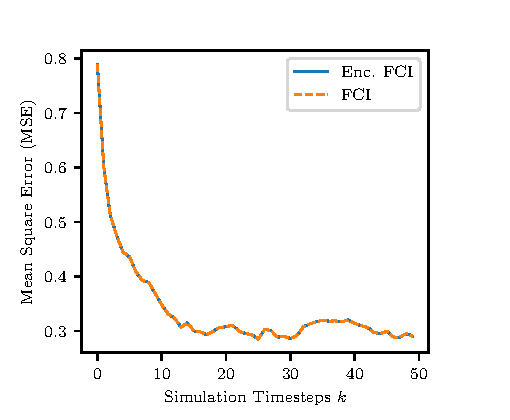
\includegraphics{figures/sim_error_plot.pdf}
    \caption{Average RMSE of encrypted and unencrypted FCI fusion over $1000$ simulations.}
    \label{fig:sim_error_plot}
\end{figure}
From the figure, we can see the expected similarity in performance between the encrypted and unencrypted FCI methods. Additionally, we note that the current recommended key length for the Paillier encryption scheme is $2048$ bits \cite{barkerRecommendationPairWiseKey2019}, easily supporting a modulus $N$ and fractional precision $\phi$ that guarantee similar performance.

% 
%  .d8888b.   .d88888b.  888b    888  .d8888b.  
% d88P  Y88b d88P" "Y88b 8888b   888 d88P  Y88b 
% 888    888 888     888 88888b  888 888    888 
% 888        888     888 888Y88b 888 888        
% 888        888     888 888 Y88b888 888        
% 888    888 888     888 888  Y88888 888    888 
% Y88b  d88P Y88b. .d88P 888   Y8888 Y88b  d88P 
%  "Y8888P"   "Y88888P"  888    Y888  "Y8888P"  
%                                               
%                                               
%                                               
% 
\section{Conclusion}\label{sec:conclusion}
In this work, we have presented a method for computing encrypted Fast Covariance Intersection homomorphically on an untrusted cloud and discussed its security guarantees. The method ensures no information leakage at the cloud, eavesdroppers or estimators and an accompanying simulation demonstrates its minimal effect on estimation performance when compared to the unencrypted algorithm. Applications include a variety of distributed fusion tasks when external fusing computations are required such as weather forecasting and vehicle localisation. Future work on the topic aims to extend the method to include multivariable encryption, hiding the dimension variable $n$, and generalising to decentralised environments where individual fusing parties are untrusted.

%%%%%%%%%%%%%%%%%%%%%%%%%%%%%%%%%%%%%%%%%%%%%%%%%%%%%%%%%%%%%%%%%%%%%%%%%%%%%%%%

% This command serves to balance the column lengths
% on the last page of the document manually. It shortens
% the textheight of the last page by a suitable amount.
% This command does not take effect until the next page
% so it should come on the page before the last. Make
% sure that you do not shorten the textheight too much.
%\addtolength{\textheight}{-11.05cm}

%%%%%%%%%%%%%%%%%%%%%%%%%%%%%%%%%%%%%%%%%%%%%%%%%%%%%%%%%%%%%%%%%%%%%%%%%%%%%%%%

% 
% 8888888b.  8888888888 8888888888 .d8888b.  
% 888   Y88b 888        888       d88P  Y88b 
% 888    888 888        888       Y88b.      
% 888   d88P 8888888    8888888    "Y888b.   
% 8888888P"  888        888           "Y88b. 
% 888 T88b   888        888             "888 
% 888  T88b  888        888       Y88b  d88P 
% 888   T88b 8888888888 888        "Y8888P"  
%                                            
%                                            
%                                            
% 
\bibliographystyle{IEEEtran}
\bibliography{bibliography/PaillierFCI}

\end{document}
